\documentclass[12pt]{article}

\usepackage[utf8]{inputenc}
\usepackage[russian]{babel}

\usepackage{amssymb}
\usepackage{amsmath}
\usepackage{amsthm}
\usepackage{xcolor}

\usepackage{indentfirst}

%\usepackage{marginnote} % this is used for notes on the right margin --- \marginnote{\footnotesize txt}

\usepackage{mathtools} % for mathclap command

%\usepackage[normalem]{ulem} % for crossing text out - \sout

% Redefining \def is impossible. I tried, but it is impossible.
%\let\def_prev\def

%%%%%%%%%%%%%%%%%%%%%%%%%%%%%%%%%%%%%%%%%%%%%%%
%           MATH OPERATORS SPACING            %
%%%%%%%%%%%%%%%%%%%%%%%%%%%%%%%%%%%%%%%%%%%%%%%

\let\existstemp\exists
\let\foralltemp\forall
\renewcommand{\exists}{\: \existstemp \:}
\newcommand{\existsonly}{\: \existstemp ! \:}
\renewcommand{\forall}{\: \foralltemp \:}

%%%%%%%%%%%%%%%%%%%%%%%%%%%%%%%%%%%%%%%%%%%%%%%
%            COMMAND SHORTHANDS               %
%%%%%%%%%%%%%%%%%%%%%%%%%%%%%%%%%%%%%%%%%%%%%%%

\newcommand{\example}{{\itshape Пример. }}
\newcommand{\equals}{\Leftrightarrow}
%\newcommand{\defi}{{\itshape Определение. }}
\newcommand{\exc}{{\bfseries Упражнение. }}
\newcommand{\norm}[1]{\| #1 \|}
\newcommand{\scal}[2]{\, < \!\! #1, #2 \!\! > \,}
\newcommand{\Sum}[2]{\underset{#1}{\overset{#2}{\sum}}}

\renewcommand{\leq}{\leqslant}
\renewcommand{\geq}{\geqslant}

%%%%%%%%%%%%%%%%%%%%%%%%%%%%%%%%%%%%%%%%%%%%%%%
%         THEOREM DEFINITION LINES            %
%%%%%%%%%%%%%%%%%%%%%%%%%%%%%%%%%%%%%%%%%%%%%%%

\newtheorem{lem}{Лемма}[section]
\newtheorem{defi}{Определение}[section]
\newtheorem{theorem}{Теорема}[section] % statement
\newtheorem{state}{Утверждение}[section] % statement

%%%%%%%%%%%%%%%%%%%%%%%%%%%%%%%%%%%%%%%%%%%%%%%
%             GRAPHICS INCLUSION              %
%%%%%%%%%%%%%%%%%%%%%%%%%%%%%%%%%%%%%%%%%%%%%%%

\usepackage{graphicx}

\setcounter{section}{4}

\begin{document}
	\title{Основы функционального анализа, второй семестр.}
	\author{Тресков Сергей Андреевич}
	\maketitle
	
	\section{Лекция}
	
	Как известно, в конечномерном пространстве все нормы являются эквивалентными. Но это отнюдь не является верным для бесконечномерных
	пространств.
	
	\example Оператор дифференцирования $\frac{d}{dx} \mathbb{L}_2(0, 1) \rightarrow \mathbb{C}_2(0, 1)$ является неограниченным. 
	Достаточно рассмотреть $\norm{sin(nx)}_{\mathbb{L}_2} \leq 1$. При воздействии на синус оператором дифференцирования, получим
	$|n \cdot cos(nx)| \geq n \cdot cos^2(nx) = n \cdot \frac{1 + cos(2nx)}{2}$.
	
	% Доразобраться
	
	\begin{theorem}
		Рассмотрим линейный оператор $A_1 : E \rightarrow F$. Если выполнены следующие условия:
		\begin{enumerate}
			\item $F$ --- полное.
			\item $D(A_1) = E_1 \subset E_2$.
			\item $\bar{E_1} \subset E_2$ (То есть $E_1$ плотно в $E_2$).
		\end{enumerate}
		То найдётся линейный оператор $A_2, D(A_2) = E_2$, такой, что: \\
		$\norm{A_2} \leq \norm{A_2}$ \\
		$A_2 |_{E_1} = A_1$
	\end{theorem}
	
	\begin{proof}
		Введём $x \in E_2, x_i \in E_1$. Пусть элементы $x_i$ образуют фундаментальную последовательность. Так как $E_1$ плотно в $E_2$,
		то найдётся элемент $x \in E_2$, являющийся пределом последовательности $x_1, ..., x_n, ...$.
		
		Воздействуем операторами $A_1$ и $A_2$ на данные элементы. Получаем:
		$$A_2 x = y$$ 
		Где $y$ --- некоторый элемент множества $E_2$. С другой стороны, мы можем x представить как предел последовательности $\{x_n\}$
		$$y = lim (y_n) = lim(A_1 x_n)$$
		Теперь рассмотрим элемент $z = \alpha x + \beta y$ и сходящуюся к нему последовательность $z_n = \alpha x_n + \beta y_n$.
		Воздействуюя оператором $A_1$ на $z_n$, получаем выражение:
		$$A_1 z_n = \alpha A_1 x_n + \beta A_1 y_n$$
		В пределе, при $n \rightarrow \infty$, равенство преобразуется следующим образом:
		$$A_2 z = \alpha A_2 x + \beta A_2 y$$
		
		Далее, покажем, что ограниченность оператора $A_1$ влечёт ограниченность оператора $A_2$. Для этого рассмотрим следующее 
		неравенство:
		
		$$\norm{A_1 x_n} \leq \norm{A_1} \cdot \norm{x_n}$$
		
		В пределе $A_1 x_n \underset{n \rightarrow \infty}{\rightarrow} A_2 x$. Тогда
		
		$$\norm{A_2 x} \leq \norm{A_1} \cdot \norm{x_n}$$
		
		Таким образом, ограниченность оператора $A_1$ влечёт ограниченность оператора $A_2$.
	\end{proof}
	
	Введём определение предела последовательности оператора. Стоит отметить, что в различной литературе данное определение может вводиться
	по-разному.
	
	\begin{defi}
		$A$ является \textbf{пределом} $A_n$, если:
		
		$$\forall x \in E, A_n x \underset{n \rightarrow \infty}{\rightarrow} A x$$
	\end{defi}
	Это определение предела не требует никакого определение нормы. В нормированных пространствах вводится еще один 
	важный термин:
	
	\begin{defi}
		Если для линейного оператора $A$ и последовательности линейных операторов $A_n$ определено соотношение:
		$$\norm{A_n - A} \rightarrow 0$$
		то $A_n$ \textbf{равномерно сходится} к $A$, что обозначается как $A_n \rightrightarrows A$.
	\end{defi}
	
	Легко показать, что равномерная сходимость всегда влечёт обычную. Действительно, рассмотрим
	$$\norm{A_n x - A x} \leq \norm{A_n - A} \cdot \norm{x} \rightarrow 0$$
	Отсюда следует $\forall x, A_n x \rightarrow A x$, что является определением сходимости линейных операторов.
	%\begin{state}
	%	Равномерная сходимость линейных операторов 
	%\end{state}
	
	В приведённых выше рассуждениях есть одна неочевидная деталь --- предел последовательности элементов не обязательно должен лежать
	в том же множестве, что и элементы последовательности. Является ли $A$, как предел $A_n$ линейным оператором?
	
	\begin{state}
		Предел последовательности линейных операторов является линейным оператором.
	\end{state}
	\begin{proof}
		Проверим, обладает ли $A$ свойствами линейного оператора. Рассмотрим вектор $z = \alpha x + \beta y$. Тогда, пользуясь линейностью
		операторов из последовательности $A_n$:
		$$ A_n \cdot z \rightarrow A \cdot z $$
		$$ \alpha A_n x + \beta A_n y \rightarrow \alpha A x + \beta A y $$
		Значит, верно равенство $A(\alpha x + \beta y) = \alpha A x + \beta A y$ и $A$ является линейным оператором.
	\end{proof}
	
	Определить ограниченность оператора $A$, исходя из свойств последовательности $A_n$ намного сложнее, но легко установим следующий
	факт:
	\begin{state}
		Если $A_n \rightarrow A$ и $\forall n, \norm{A_n} \leq C$, где $C$ --- некоторая константа, то оператор $A$ является ограниченным.
	\end{state} 
	\begin{proof}
		Очевидно. {\color{gray}Sorry, но я и так умаялся предыдущее доказательство писать, а оно тоже очевидное.}
	\end{proof}
	
	\example $P_n : l_2 \rightarrow l_2$ --- оператор проектирования на n-мерное подпространство.
	$$P_n : (x_1, \dots , x_n, x_{n+1}, \dots) \longmapsto (x_1, \dots, x_n, 0, 0, 0, \dots)$$
	Рассматривая свойства пространства $l_2$, легко понять, что $P_n \rightarrow I$. Действительно, так как $x_n$ --- элементы 
	сходящегося ряда, то $lim (x_n) \rightarrow 0$. Таким образом, норма <<хвоста>> ряда будет стремиться к нулю.
	%\marginnote{\footnotesize I --- тождественный оператор}[-1.5cm]
	Но, в то же время, равномерной сходимости не достигается: $\norm{P_n - I} = 1$. Следовательно, обычная сходимость не влечёт
	равномерную.
	
	\exc Пусть $A_n \rightrightarrows A, B_n \rightrightarrows B$. Доказать $A_n B_n \rightrightarrows A B$. 
	(Разумеется, доказывается данное утверждение в предположении, что композиция $A B$ существует, то есть совпадают область определения
	A и множество значений B.)
	
	\begin{state}
		Рассмотрим последовательность $A_n : E \rightarrow F$. Утверждается, что, если $F$ --- плотное, то пространство 
		ограниченных линейных операторов $\{A_n\}$ образует полное нормированное пространство.
	\end{state}
	\begin{proof}
		Возьмём $A_n$ --- фундаментальную последовательность, тогда $\norm{A_n - A_m} \rightarrow 0$, отсюда следует, что 
		$A_n \cdot x$ --- фундаментальная последовательность и, так как $F$ --- полное множество, она имеет предел, который
		мы обозначим за $A \cdot x$ ($\forall x A_n \cdot x \rightarrow A \cdot x$).
		
		\textbf{Линейность.} Ранее уже было доказано, что предел последовательности линейных операторов также является линейным
		оператором.
		
		\textbf{Ограниченность.} Так как последовательность является фундаментальной, можем ограничить норму разности её элементов 
		константой.
		$$\norm{A_n - A_m} \leq 1$$
		Тогда, применяя неравенство треугольника, легко приходим к доказательству ограниченности оператора:
		$$\norm{A_n} \leq 1 + \norm{A_m}$$
		
		\textbf{Равномерная сходимость.} По определению фундаментальной последовательности:
		$$
			\norm{A_n - A_m} \rightrightarrows 0 \overset{df}{\equals} 
			\forall varepsilon > 0 \exists N_0 \forall m, n \geq N_0 \norm{A_n - A_m} < \varepsilon
		$$
		В силу сходимости $A_n \rightarrow A$, получаем, в таких же обозначениях:
		$$ \norm{A_n - A} \leq \varepsilon $$
		Данное неравенство при $\varepsilon \rightarrow 0$ является определением равномерной сходимости.
		
		Таким образом, $\{A_n\}$ обладает всеми свойствами, нужными для того, чтобы пространство являлось полным, что и требовалось 
		доказать.
	\end{proof}
	
	\begin{defi}
		Если для полного пространства $F$ и операторов $A_n : E \rightarrow F$ имеет место предельное соотношение
		$$\Sum{n=1}{N} A_n \underset{N \rightarrow \infty}{\rightarrow} A,$$
		то оператор $A = \Sum{n=1}{\infty} A_n$ называют \textbf{операторным рядом}.
	\end{defi}
	
	Определим для подобного ряда критерий Коши (критерий сходимости фундаментальной последовательности):
	$$\forall \varepsilon > 0 \exists N(\varepsilon) m > n > N(\varepsilon) \norm{ \Sum{n}{m} A_i } < \varepsilon$$
	
	Операторный ряд является одним из способов построения функции от операторов. Но данным способом могут быть выражены только степенные
	функции.
	
	\example Пусть $A$ --- ограниченный линейный оператор. Тогда ряд 
	$$\Sum{n = 0}{\infty} \frac{(A^n}{n!}$$
	сходится, так как $\norm{A^n} \leq \norm{A}^n$, а ряд $\Sum{n=0}{\infty} \frac{\norm{A}^n}{n!}$ ничем не отличается от ряда
	$\Sum{n=0}{\infty} \frac{t^n}{n!}$, обладающего радиусом сходимости $R = \infty$.
	
	\subsection*{Обратный оператор}
	
	Чтобы существовало обратное отображение $A^{-1}$, необходима инъективность оператора $A$. Более формально это записывается так: \\
	Пусть $E : A \rightarrow F$ и $A$ --- инъективен $\Rightarrow \exists A^{-1}, D(A^{-1}) = Im(A)$.
	
	\begin{state}
		$A^{-1}$ аддитивен и линеен.
	\end{state}
	\begin{proof}
		\textbf{Аддитивность.} Рассмотрим вектора $y \in Im(A), z \in Im(A)$, тогда по линейности $A$, $y + z \in Im(A)$.
		Определим вектор $x$:
		$$x = A^{-1}(y + z) - A^{-1} y - A^{-1} z$$
		Воздействуем на него оператором A, учитывая, что $A A^{-1} = I$.
		$$Ax = I(y + z) - I y - I z = 0$$
		Таким образом, из линейности оператора $A$, $x = 0$, что доказывает аддитивность обратного оператора.
		
		\textbf{Однородность.} Опять же, рассмотрим $y \in Im(A)$ и определим вектор $x$:
		$$ x = A^{-1}(\lambda y) - \lambda A^{-1} y $$
		$$ Ax = \lambda y - \lambda y = 0 $$
		Следовательно, $x = 0$, поэтому $A^{-1}$ однородно.
		
		Доказаны аддитивность и однородность $\Rightarrow$ оператор $A^{-1}$ линеен.
	\end{proof}
	
	Ограниченность оператора $A$ отнюдь не влечёт ограниченность $A^{-1}$. Но именно для такого случая предусмотрены банаховы 
	пространства:
	
	\begin{theorem}
		(Без доказательства) Если $A$ --- линеен, ограничен и отображает полное нормированное пространство на полное нормированное
		пространство, то $\exists A^{-1}$ --- линейный и ограниченный оператор.
	\end{theorem}
	
	Пусть $A$ --- линейный оператор и $$\exists m > 0 : \forall x \norm {Ax} \geq m \cdot \norm{x}$$
	Это будет означать, что $A$ --- инъективный оператор, так как
	$$\norm{A(x-y)} \geq m \cdot \norm{x - y}$$
	Из этого неравенства следует, что, если $Ax = Ay$, то $x = y$. И, разумеется, инъективность оператора будет означать его
	обратимость.
	
	В таких условиях, оператор $A^{-1}$ будет ограниченным:
	$$ x = A^{-1} y $$
	$$ \norm{A^{-1} y} \leq \frac{1}{m} \norm{y} $$
	И это, в силу определения нормы оператора, означает $$\norm{A} \leq \frac{1}{m}$$
	
	\begin{theorem}
		Пусть $F$ --- полное пространство, $A : F \rightarrow F$ --- линейный оператор, $\norm{A} \leq 1$.
		Тогда оператор $I_F - A$ является обратимым, причём обратный оператор определяется как:
		$$
			(I_F - A)^{-1} = \Sum{0}{\infty} A^n
		$$
	\end{theorem}
	Стоит отметить, что ряд $\Sum{0}{\infty} A^n$ будет сходиться, так как $\norm{A} \leq 1$. Более того, сумма этого ряда определяется
	как сумма бесконечно убывающей геометрической прогрессии.
	\begin{proof}
		Умножим $(I_F - A)$ на частичную сумму ряда $\Sum{0}{N} A^n$:
		$$ (\Sum{0}{N} A^n ) \cdot (I_F - A) = I_F - A^{N+1} \rightarrow I_F $$
		Взяв $N \rightarrow \infty$ превратим предел в равенство; умножим обе части уравнения на $(I_F - A)^{-1}$. Получаем
		$$ \Sum{0}{\infty} A^n = (I_F - A)^{-1} $$
		что совпадает с формулой, указанной в теореме.
	\end{proof}
	
	\begin{state}
		A --- обратим, $\Delta$ --- ограниченный оператор, $\norm{\Delta} \leq \frac{1}{\norm{A^{-1}}}$, тогда оператор 
		$A + \Delta$ будет обратимым.
	\end{state}
	\begin{proof}
		Вынесем $A$ за скобки:
		$$ A + \Delta = A \cdot \underbrace{(I + A^{-1} \cdot \Delta)}_{\text{Обратимо по предыдущей теоремы.}} $$
	\end{proof}
	
	\subsection*{Спектр линейного оператора}
	
	Рассмотрим $A : F \rightarrow F$:%, $F$ --- плотное пространство.
	$$(A - \lambda \cdot I) = \lambda \cdot (\frac{A}{\lambda	} - I)$$
	Как видно из ранее приведённых теорем, оператор $(A - \lambda \cdot I)$ будет обратимым при достаточно больших значениях $\lambda$.
	
	Запишем все группы $\lambda$, определяемые свойствами оператора $(A - \lambda \cdot I)$
	
	\begin{center}
		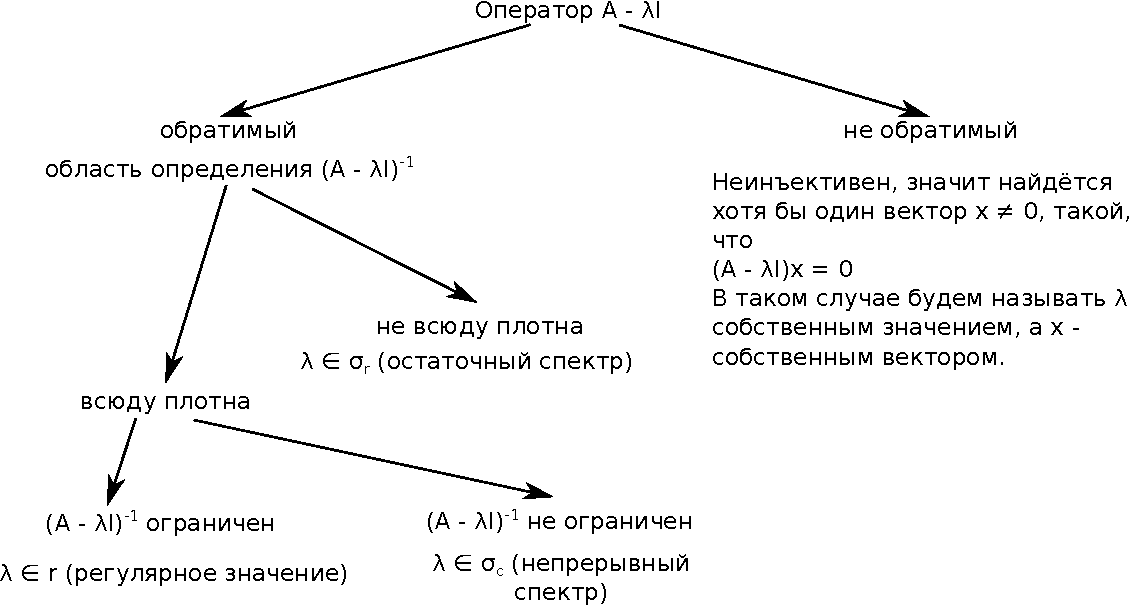
\includegraphics[width=1.0\linewidth]{Lectures-6-spectrum_scheme.pdf}\\
	\end{center}
	
	Для каждого $\lambda \in r(A)$ определяется ограниченный, с всюду плотной областью определения оператор
	$$ R_{\lambda} = (A - \lambda I)^{-1}$$
	Где $R_{\lambda}$ называется \textbf{резолентным оператором}. \\
	Также отметим равенство, верное для любого линейного оператора:
	$$
		\overbrace{r(A)}^{ \mathclap{\text{Регулярные значения $A$}} } \cup 
		\underbrace{\sigma_1 (A) \cup \sigma_2 (A) \cup \sigma_3 (A)}_{\text{Спектр $A$}} = 
		r(A) \cup \sigma(A) = \mathbb{C}
	$$
\end{document}